\documentclass{beamer}

\usetheme{Madrid}
%\setbeamertemplate{footline}[frame number]
\setbeamertemplate{navigation symbols}{}

%----------------------------------------------------
%The following packages add LaTeX commands that make formatting and writing math easier

\usepackage{graphicx}  % Include figure files
\usepackage{subcaption}
\usepackage{multirow}

\usepackage[T1]{fontenc}
\usepackage{dcolumn}   % Align table columns on decimal point

\usepackage{physics}
\usepackage{siunitx}
\usepackage{mathtools}
\usepackage{bm}        % bold math
\usepackage{amsfonts}  % Common math fonts
\usepackage{amsmath}   % Common math functions
\usepackage{amssymb}   % Common math symbols
\usepackage{esint}
\usepackage{mathrsfs}
\usepackage{slashed}   % Feynman slash

%----------------------------------------------------
%The following custom commands simplify commonly used LaTeX commands

%Parentheses and Brackets
\newcommand{\paren}[1]{\left( #1 \right)}
\newcommand{\bracket}[1]{\left[ #1 \right]}

%Quantum Mechanics
\newcommand{\dg}{^\dagger}
\newcommand{\exv}[1]{\left\langle #1 \right\rangle}

%Derivatives

\newcommand{\pdtwo}[2]{\frac{\partial^2 #1}{\partial #2 ^2}}
\newcommand{\fdtwo}[2]{\frac{d^2 #1}{d #2 ^2}}

%Fonts
\newcommand{\bb}{\mathbf}
\newcommand{\mrm}{\mathrm}
\newcommand{\bi}{\boldsymbol}

\newcommand{\mcal}{\mathcal}
\newcommand{\mbb}{\mathbb}
\newcommand{\mscr}{\mathscr}
\newcommand{\mfrak}{\mathfrak}

%Equation
\newcommand{\eq}[1]{\begin{equation} #1 \end{equation}}

%Matrices

\newcommand{\sigx}{\left( \begin{array}{cc} 0 & 1\\ 1 & 0 \end{array}\right)}
\newcommand{\sigy}{\left( \begin{array}{cc} 0 & -i\\ i & 0 \end{array}\right)}
\newcommand{\sigz}{\left( \begin{array}{cc} 1 & 0\\ 0 & -1 \end{array}\right)}

\newcommand{\mymatrix}[1]{\begin{pmatrix} #1 \end{pmatrix}}

%---------------------------------------------------



\title[Entangled Relativity]{Dynamics around Charged Black Holes\\
in Entangled Relativity}
\author[Arnaud Crepinge]{Arnaud Crepinge}
\institute[]{Supervised by Olivier Minazzoli\\
Observatoire de la Côte-d'Azur}
\date{July 10, 2026}

\begin{document}

\begin{frame}
  \titlepage
\end{frame}

\begin{frame}{Plan}
  \tableofcontents
\end{frame}

\section{Introduction}
\begin{frame}{Introduction}
    The two principles of General Relativity:
    \begin{itemize}
        \item General covariance
        \item Equivalence principle
    \end{itemize}

    Conventions: $(-,+,+,+)$ metric signature and $c=\hbar=G=4\pi\varepsilon_0 = 1$ natural system of units.

\end{frame}

\section{General Relativity}
\subsection{The theory of General Relativity}
\begin{frame}{General Relativity}

Einstein-Hilbert action:

\begin{equation}
    S\bracket{g, \Psi} = \int\paren{\frac{R}{2\kappa} + \mcal L_m} \sqrt{|g|}\mrm d^4x
\end{equation}

Einstein field equations:

\begin{eqnarray}
    R_{\mu\nu} - \frac{1}{2}Rg_{\mu\nu} = \kappa T_{\mu\nu}
\end{eqnarray}

with $T_{\mu\nu} = -\frac{2}{\sqrt{|g|}}\pdv{(\sqrt{|g|}\mcal L_m)}{g^{\mu\nu}}$.
  
\end{frame}

\subsection{Reissner-Nordström Background}
\begin{frame}{Reissner-Nordström Black Hole}

    Reissner-Nordström solution:

    \begin{align}
        \mrm ds^2 = &-\paren{1 - \frac{r_+}{r}}\paren{1 - \frac{r_-}{r}}\mrm dt^2 \notag\\
        & + \paren{1 - \frac{r_+}{r}}^{-1}\paren{1 - \frac{r_-}{r}}^{-1}\mrm dr^2 \notag\\
        & + r^2 \paren{\mrm d\theta^2 + \sin^2\theta \mrm d\varphi^2}
    \end{align}

    Horizons:

    \begin{equation}
        r_\pm = M \pm \sqrt{M^2 - Q^2}
    \end{equation}

    The solution exists for $|Q|/M \leq 1$.
  
\end{frame}

\section{Entangled Relativity}
\subsection{The theory of Entangled Relativity}
\begin{frame}{Entangled Relativity}

    Action of Entangled Relativity:

    \begin{equation}
        S\bracket{g, \Psi} = \int \frac{\mcal L_m^2}{R}\sqrt{|g|}\mrm d^4x
    \end{equation}

    Field equations:

    \begin{equation}
        R_{\mu\nu} - \frac{1}{2}Rg_{\mu\nu} = -\frac{R}{\mcal L_m}T_{\mu\nu}+\frac{R^2}{\mcal L_m^2}\paren{\nabla_\mu\nabla_\nu - g_{\mu\nu}\square}\frac{\mcal L_m^2}{R^2}
    \end{equation}
  
\end{frame}

\begin{frame}{Scalar-Tensor form of Entangled Relativity}

  
\end{frame}

\subsection{Charged Black Holes in Entangled Relativity}
\begin{frame}{Charged Black Holes in Entangled Relativity}
  
    Charged black hole solution of ER:

    \begin{align}
        \mrm ds^2 = &-\paren{1 - \frac{r_+}{r}}\paren{1 - \frac{r_-}{r}}^{15/13}\mrm dt^2 \notag\\
        &+ \paren{1 - \frac{r_+}{r}}^{-1}\paren{1 - \frac{r_-}{r}}^{-7/13}\mrm dr^2 \notag\\
        &+ r^2\paren{1 - \frac{r_-}{r}}^{6/13}\paren{\mrm d\theta^2 + \sin^2\theta \mrm d\varphi^2}
    \end{align}

    Scalar Field:

    \begin{equation}
        \phi = \paren{1 - \frac{r_-}{r}}^{-4/13}
    \end{equation}

\end{frame}

\begin{frame}{Conformal Transformation}
    
    Einstein frame obtained by:

    \begin{equation}
        g_{\mu\nu} \mapsto \tilde g_{\mu\nu} = \phi g_{\mu\nu} 
    \end{equation}

    New solution:

    \begin{align}
        \mrm d\tilde s^2 = &-\paren{1 - \frac{r_+}{r}}\paren{1 - \frac{r_-}{r}}^{11/13}\mrm dt^2 \notag\\
        &+ \paren{1 - \frac{r_+}{r}}^{-1}\paren{1 - \frac{r_-}{r}}^{-11/13}\mrm dr^2 \notag\\
        &+ r^2\paren{1 - \frac{r_-}{r}}^{2/13}\paren{\mrm d\theta^2 + \sin^2\theta \mrm d\varphi^2}
    \end{align}
\end{frame}

\begin{frame}{Domain of Validity of the Solution}

    Horizons:

    \begin{align}
        r_- &= \frac{13}{11}\paren{M - \sqrt{M^2 - \frac{11}{12}Q^2}}\\
        r_+ &= M + \sqrt{M^2 - \frac{11}{12}Q^2}
    \end{align}

    Two conditions:
    \begin{itemize}
        \item Real-valued radii: $|Q|/M \leq \sqrt{12/11}$
        \item Inner horizon lower than outer horizon: $r_- \leq r_+$
    \end{itemize}

    Solution exists for $|Q|/M \leq \sqrt{143/132}$.
    
\end{frame}

\begin{frame}{Areal Radius}

    Areal radius:

    \begin{equation}
        \rho_\mrm{GR} = r_\mrm{GR},\ \ \ \rho_\mrm{ER} = r_\mrm{ER}\paren{1 - \frac{r_-}{r_\mrm{ER}}}^{1/13}
    \end{equation}

    \begin{figure}
        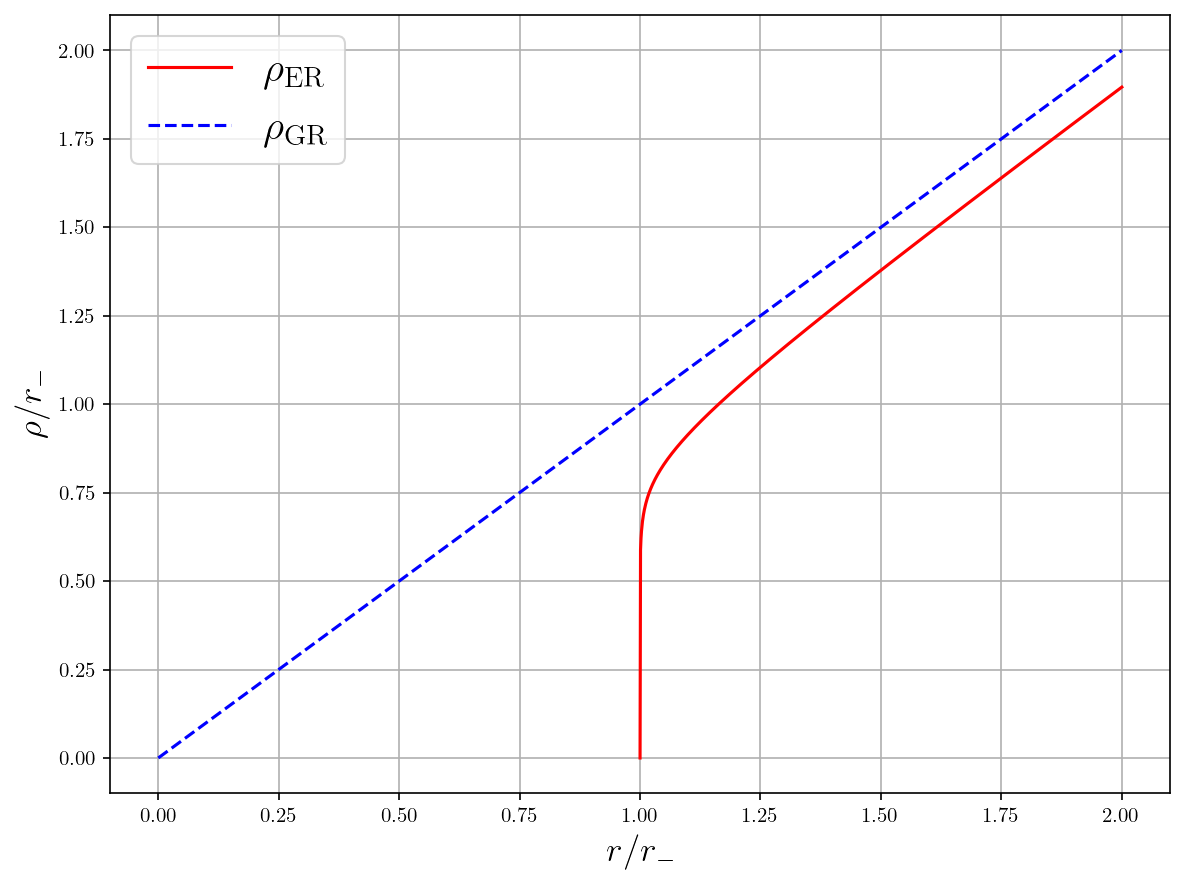
\includegraphics[width=0.6\linewidth]{images/rho.png}
    \end{figure}
    
\end{frame}

\section{Results}
\subsection{Null Geodesics Analysis}
\begin{frame}{Null Geodesics Analysis}
  
\end{frame}

\begin{frame}{Null Geodesics Analysis}
  
\end{frame}

\subsection{Timelike Geodesics Analysis}
\begin{frame}{Timelike Geodesics Analysis}
  
\end{frame}

\begin{frame}{Timelike Geodesics Analysis}
  
\end{frame}

\subsection{Black Hole Phenomenology}
\begin{frame}{Black Hole Phenomenology}
  
\end{frame}

\section{Conclusion}
\begin{frame}{Conclusion}
  
\end{frame}

\end{document}